\documentclass[chi_draft]{sigchi}

% Use this command to override the default ACM copyright statement
% (e.g. for preprints).  Consult the conference website for the
% camera-ready copyright statement.

%% EXAMPLE BEGIN -- HOW TO OVERRIDE THE DEFAULT COPYRIGHT STRIP -- (July 22, 2013 - Paul Baumann)
% \toappear{Permission to make digital or hard copies of all or part of this work for personal or classroom use is      granted without fee provided that copies are not made or distributed for profit or commercial advantage and that copies bear this notice and the full citation on the first page. Copyrights for components of this work owned by others than ACM must be honored. Abstracting with credit is permitted. To copy otherwise, or republish, to post on servers or to redistribute to lists, requires prior specific permission and/or a fee. Request permissions from permissions@acm.org. \\
% {\emph{CHI'14}}, April 26--May 1, 2014, Toronto, Canada. \\
% Copyright \copyright~2014 ACM ISBN/14/04...\$15.00. \\
% DOI string from ACM form confirmation}
%% EXAMPLE END -- HOW TO OVERRIDE THE DEFAULT COPYRIGHT STRIP -- (July 22, 2013 - Paul Baumann)

% Arabic page numbers for submission.  Remove this line to eliminate
% page numbers for the camera ready copy
% \pagenumbering{arabic}

% Load basic packages
\usepackage{balance}  % to better equalize the last page
\usepackage{graphicx} % for EPS, load graphicx instead 
\usepackage{float}
\usepackage[caption = false]{subfig}
\usepackage[T1]{fontenc}
\usepackage{txfonts}
\usepackage{mathptmx}
\usepackage[pdftex]{hyperref}
\usepackage{color}
\usepackage{booktabs}
\usepackage{textcomp}
\usepackage[inline]{enumitem}
\usepackage{xspace}
\usepackage[table,xcdraw]{xcolor}
% Some optional stuff you might like/need.
\usepackage{microtype} % Improved Tracking and Kerning
% \usepackage[all]{hypcap}  % Fixes bug in hyperref caption linking
\usepackage{ccicons}  % Cite your images correctly!
% \usepackage[utf8]{inputenc} % for a UTF8 editor only

%OUR OWN REF PACKAGES
\usepackage{hyperref} %doublecheck the need for this one, this tex file has a global style for URL
\usepackage{cleveref}
\usepackage{csquotes}
%\creflabelformat{figure}{(#2#1#3)}


% If you want to use todo notes, marginpars etc. during creation of your draft document, you
% have to enable the "chi_draft" option for the document class. To do this, change the very first
% line to: "\documentclass[chi_draft]{sigchi}". You can then place todo notes by using the "\todo{...}"
% command. Make sure to disable the draft option again before submitting your final document.
\usepackage{todonotes}

% Variable definitions
\newcommand{\pinch}{\emph{Pinch}\xspace}
\newcommand{\swipe}{\emph{Swipe}\xspace}
\newcommand{\throw}{\emph{Throw}\xspace}
\newcommand{\tilt}{\emph{Tilt}\xspace}

\newcommand{\ts}{\textsuperscript}

% Paper metadata (use plain text, for PDF inclusion and later
% re-using, if desired).  Use \emtpyauthor when submitting for review
% so you remain anonymous.
\def\plaintitle{Insert long clever title here}
\def\plainauthor{First Author, Second Author, Third Author,
  Fourth Author, Fifth Author, Sixth Author}
\def\emptyauthor{}
\def\plainkeywords{Authors' choice; of terms; separated; by
  semicolons; include commas, within terms only; required.}
\def\plaingeneralterms{Documentation, Standardization}

% llt: Define a global style for URLs, rather that the default one
\makeatletter
\def\url@leostyle{%
  \@ifundefined{selectfont}{
    \def\UrlFont{\sf}
  }{
    \def\UrlFont{\small\bf\ttfamily}
  }}
\makeatother
\urlstyle{leo}

% To make various LaTeX processors do the right thing with page size.
\def\pprw{8.5in}
\def\pprh{11in}
\special{papersize=\pprw,\pprh}
\setlength{\paperwidth}{\pprw}
\setlength{\paperheight}{\pprh}
\setlength{\pdfpagewidth}{\pprw}
\setlength{\pdfpageheight}{\pprh}

% Make sure hyperref comes last of your loaded packages, to give it a
% fighting chance of not being over-written, since its job is to
% redefine many LaTeX commands.
\definecolor{linkColor}{RGB}{6,125,233}
\hypersetup{%
  pdftitle={\plaintitle},
% Use \plainauthor for final version.
%  pdfauthor={\plainauthor},
  pdfauthor={\emptyauthor},
  pdfkeywords={\plainkeywords},
  bookmarksnumbered,
  pdfstartview={FitH},
  colorlinks,
  citecolor=black,
  filecolor=black,
  linkcolor=black,
  urlcolor=linkColor,
  breaklinks=true,
  hypertexnames=false
}

% create a shortcut to typeset table headings
% \newcommand\tabhead[1]{\small\textbf{#1}}

% End of preamble. Here it comes the document.
\begin{document}

\title{\plaintitle}

\numberofauthors{3}
\author{%
  \alignauthor{Leave Authors Anonymous\\
    \affaddr{for Submission}\\
    \affaddr{City, Country}\\
    \email{e-mail address}}\\
  \alignauthor{Leave Authors Anonymous\\
    \affaddr{for Submission}\\
    \affaddr{City, Country}\\
    \email{e-mail address}}\\
  \alignauthor{Leave Authors Anonymous\\
    \affaddr{for Submission}\\
    \affaddr{City, Country}\\
    \email{e-mail address}}\\
}

\maketitle

% !TEX root = ../paper.tex
\begin{abstract}
\todo[inline]{Write abstract}

\todo{Add section numbers to each section because of references to certain sections of the paper}

\end{abstract}


\category{H.5.m.}{Information Interfaces and Presentation
  (e.g. HCI)}{Miscellaneous} \category{See
  \url{http://acm.org/about/class/1998/} for the full list of ACM
  classifiers. This section is required.}{}{}

\keywords{\plainkeywords}

% !TEX root = ../paper.tex
\section{Introduction} \label{sec:introduction}
The evolution of ways people interact with the digital is noteworthy considering the short life-span of computing. How we use our devices, which devices we use, and the context in which we use them has been continually under transformation. From portable personal computers, originally considered mostly for specialized field applications, such accountancy, military use, or for sales representatives, which addressed mobility of a person's workspace, to modern hand-held devices which presented, their users, such degree of freedom that ultimately workspaces are starting to fade. This expansion has not only increased mobile computing due to greater convenience, but also made it widespread.\cite{Francis:1997} \\

As numerous divergent devices are being adopted in different domains and context, cross-device interaction is currently becoming more important and relevant, as people take their hand-held devices into situations where other technologies are active. This ubiquitous presence of devices means that it can be leverage to enhance everyday situations in all kind of places. Imagine if a public display can morph from one-way broadcast device that merely show visual content to a two-way interaction device that provides more engaging and immersive experience. Given this emergence of cross-device communication opportunities prompts a need to understand how different interaction techniques perform in use, e.g. in terms of how easily, quickly and accurately, or in terms of how enjoyable or satisfying it's it to interact in this way. \\

Research in the area of cross-device interaction has been trying to keep up with the changing trends, earliest examples are in the late 90's, within ubiquitous computing, with Rekimoto's work,  he argued for, what he called, multi computed user interface and that interaction technique must overcome the boundaries among devices in multi-device settings\cite{Rekimoto:1998}.

Recent HCI research has focused on how to include in cross-device interaction an more natural modality contributing to what should be know as cross-device natural user interaction.  Some researchers used spatial information \cite{Marquardt:2011, Marquardt:2012}, others used touch \cite{Seifert:2012}, or combined touch with air gestures \cite{Bragdon:2011} . But we still have limited understanding of how to design cross-device natural user interaction techniques and also we are missing on quantitative studies of the aforementioned.\\

Inspired by the opportunities presented of such challenges, this paper reports on a quantitative study between four different cross-device natural user interaction techniques for data transfer between hand-held device and large displays.

We discover that out of the four techniques we developed and implemented, \swipe was the most precise and effective technique, which could be used to create more interesting and effective natural user interfaces with. We uncover that the need for precision comes at a great cost in regards to effectiveness, and should be side-stepped\todo{contrast this with any other that was strongest at some aspect?? also, be clear about what you mean by effective.} if possible while designing and implementing the application.  


% !TEX root = ../paper.tex
\section{Related work} \label{sec:relatedwork}

Public displays is an inherently visual medium as such graphics and animations are increasingly used to visualize data, however the general case is the presented data can only be viewed and not interacted with. A change from non-interactive information broadcasters to active medium may be beneficial. 
Combining this with the recent trend of increased number of hand-held device per capita an opportunity for new cross-device applications in public space arises, providing new opportunities for exploring cross-device interaction (CDI), in this context.
As such possibility are presented researchers naturally acted on them.

In historic perspective, one of the earliest working cross-device applications is by Myers et al. \cite{Myers:2001}. 
One of the applications realized within their \emph{Pebbles project} is SlideShow Commander that utilized Personal Devices Assistants (PDA) to control a PowerPoint presentation runny on other computer or laptop.
It was possible not just moving between slides, but also scribbling and writing on the PDA slides, while annotations are shown on the presentation for the audience. 
However the idea of cross-device have deeper roots in ubiquitous computing. Rekimoto's work \emph{pick-and-drop technique} is one of the earliers examples for exploring technique that spawns between multiple devices. The technique "allows a user to pick up an object on a display and drop it on another display as if he/she were manipulating a physical object." \cite{Rekimoto:1997}. 
These two early work examples, even though in different fields, are entwined and would set a foundation for future research work.\\

An example of such research is that of Sebastian Boring's who not only build an cross-device application but explored the implications of different techniques on it. In \emph{Shoot and Copy}, Boring et al. \cite{Boring:2007} explored the transfer of data from a large public display onto a mobile device.
They created a method of transferring data from a large screen by using the camera on the mobile device.
The user would take a picture of whatever content they were interested in, after which the application would query the content server with the picture taken from the user.
Through visual analyses, the content server would determine what content the user was interested in and would return that content to them.
They show that there is a need for enabling data exchange between mobile devices and public displays.
In \emph{Scroll, Tilt or Move It}, Boring et al. \cite{Boring:2009} investigated cross device interaction between large displays and mobile phones.
More specifically, he investigated three different interaction techniques in order to continuously control a pointer on a large screen from a mobile device.
\emph{Move} and \emph{Tilt}, two of the three interaction techniques, enabled faster selection time compared to the last one, \emph{Scroll}, but at the cost of higher error rates.
They showed that different interaction techniques have certain strengths and weaknesses, and depending on the context and use, certain techniques can be used rather than other. 

Boring's idea of how to control a public display is only one side of cross-device, a different idea is about a collaboration surface made from multiple devices and it's greatly presented with
\emph{JuxtaPinch} by Nielsen et al. \cite{Nielsen:2014}, they investigate the  use of multiple device together, by allowing a number of devices being put next to each other and ``pinched'' together to form a larger collaborative workspace.
Expanding on this idea of common workspace was moving away from using multiple devices to build one large mixed device. Schmidt et al. proposed a cross-device interaction style for mobiles and surfaces where one can use multiple phones to interact with a digital surface.
The researchers point out that \emph{``natural forms of interaction have evolved for personal devices that we carry with us (mobiles) as well as for shared interactive displays around us (surfaces) but interaction across the two remains cumbersome in practice''} \cite{Schmidt:2012}; so in order to overcome this they propose to use mobiles as tangible input on the surface in a stylus like fashion.

A combination of the ideas above is presented by Skov et al. \cite{Skov:2015} illustrate six different cross-device interaction techniques for the case of card playing in \emph{Investigating Cross-Device Interaction techniques}.
A player can see their own cards on their phone and use three different techniques for playing a card from the handheld to the tablet, which is placed on a table.
In the other direction, i.e. when drawing a card, the player also has three techniques to choose from.
The usability study aims to quantitatively evaluate each of the techniques and showed that there is a difference in time and number of errors between the techniques. 
They recorded two types of errors, namely, interaction errors and play errors.
The number of interaction errors shows how difficult it is for a user to perform a given technique while play errors represent the errors related to the game and is recorded when the user plays a wrong card.
The difference in interaction errors is apparent, especially between two of the techniques for playing a card.

While the two paragraphs above ilustrated two different idea movements in cross-device, a common area of interest they have is the question of data transfer between devices.
Hamilton and Wigdor's  work \cite{Hamilton:2014} aggregate much of the works above and clearly articulate the data transfer. In \emph{Conductor} they create a prototype framework for cross-device applications by combining a number of interactions techniques for data transfer, chaining tasks, and managing interactions sessions.
Data transfer is a challenge and as such there are different approaches for solution. Marquardt et al. \cite{Marquardt:2012} study cross-device interaction on tablets with a extra natural modality, by involving spatial information - proxemics.Based on the constructs of f-formation and micro-mobility and co-present collaboration, they build their prototype with the idea of support for fluid and minimally disruptive interaction in document transfer. 
Bragdon et al.\cite{Bragdon:2011} propose using a combination of air gestures and touch.They aim to design, implement and test a system that allows a group of users to interact using air gestures and touch gestures. The purpose is to increase control, support democratic access, and share items across multiple personal devices such as smartphones and laptops where the primary design goal is fluid, democratic sharing of content on a common display.


% !TEX root = ../paper.tex
\section{Interaction techniques} \label{sec:techniques}
We have four techniques named \swipe, \tilt, \throw, and \pinch.
Our techniques all make use of some combination of pointing in mid-air and touch gestures on the smartphone screen.
Mid-air pointing is achieved by using the Microsoft Kinect for Windows which uses a depth camera making it possible to track a user's hand in mid-air.
A smartphones has an accelerometer and a touchscreen, former making it possible to detect motion input and the latter makes it possible to detect contact between e.g. a finger and the screen.
These technologies are, in combination with each other, used to recognize the four techniques described in this section. 

\begin{table}[H]
	\centering
	\begin{tabular}{|p{0.2\columnwidth}|p{0.7\columnwidth}|}
		\hline
		\rowcolor[HTML]{9B9B9B} 
		\textbf{Criteria} & \textbf{Description} \\ \hline
		Number of hands & There must be both one-handed and two-handed techniques. \\ \hline
		Previously used & To avoid designing and testing a set of novel techniques, we had the criterion that all techniques must have been used by others before we would use them. \\ \hline
		Complexity & The techniques must differ in their complexity and therefore we included techniques with different amount of steps. \\ \hline
		Natural feel & There must be a natural feel to the techniques in some way. \\ \hline
		Time & The time it takes to perform the different techniques must be different. \\ \hline
	\end{tabular}
	\caption{This table describes the set of criteria we had }
	\label{tab:techniqueCriteria}
\end{table}
%Two-handed techniques which are techniques that require both hands.

Before designing and implementing the experiment we had to find a suitable set of techniques and since the purpose of our experiment is to compare the techniques against each other, we searched for different techniques in related work.
The idea was to find a set of diverse techniques with different criteria.
The different criteria that we used are described in \Cref{tab:techniqueCriteria}.

What we ended up with was four interaction techniques we found were either completely copied as described in the related work or a combination of techniques to fit our experimental study.
In the following we explain why these four techniques were chosen and how they should be performed.

The \swipe technique (\Cref*{fig:swipeTechnique}) is used by Bragdon et al. \cite{Bragdon:2011} in Code Space, a system using the Kinect and smartphones to support developer meetings. 
Bragdon et al. describes the technique as: \emph{``cross-device interaction with touch and air pointing''} and the swipe motion is described as \emph{``flicking up on the touch screen''}. 
This technique was chosen because of its simplistic design and the low level of complexity.
Only one hand is needed and the amount of effort and time required to execute this technique is minimal compared to other techniques.
\swipe is copied exactly as described in \cite{Bragdon:2011}.
The \swipe technique is performed by 
\begin{enumerate*}[label=\itshape\roman*\upshape)]
	\item{pointing at a target on the large display with the phone in a stretched arm, and}
	\item{making a forwards swipe motion with the thumb on the phone's screen (\cref{fig:swipeTechnique}).}
\end{enumerate*}

The \tilt technique (\Cref{fig:tiltTechnique}) is used in a collaborative application by Lucero et al. \cite{Lucero:2012} to transfer an object from a large display to the user's smartphone.
Boring et al. uses the a tilt technique in \cite{Boring:2009} when moving a pointer on a display using a phone and though not the same application, the execution of the technique is the same.
We chose this technique because it is one handed, relatively low complexity, and much like the \swipe it is generally easy to use.
When the direction is reversed, \tilt is an exact copy of the way Lucero et al. describes the technique.
The \tilt technique is performed by 
\begin{enumerate*}[label=\itshape\roman*\upshape)]
	\item{pointing at a target on the large display with the phone in a stretched arm, and}
	\item{making a forwards tilt with the phone (\cref{fig:tiltTechnique}).}
\end{enumerate*}

\begin{figure}[H]
\subfloat[]{\includegraphics[width = 1\columnwidth]{images/Swipe.jpg}\label{fig:swipeTechnique1}}
\caption{
	\protect\subref{fig:swipeTechnique1} The \swipe technique is performed by using the thumb to swipe.
}
\label{fig:swipeTechnique}
\end{figure}

\begin{figure}[H]
\subfloat[]{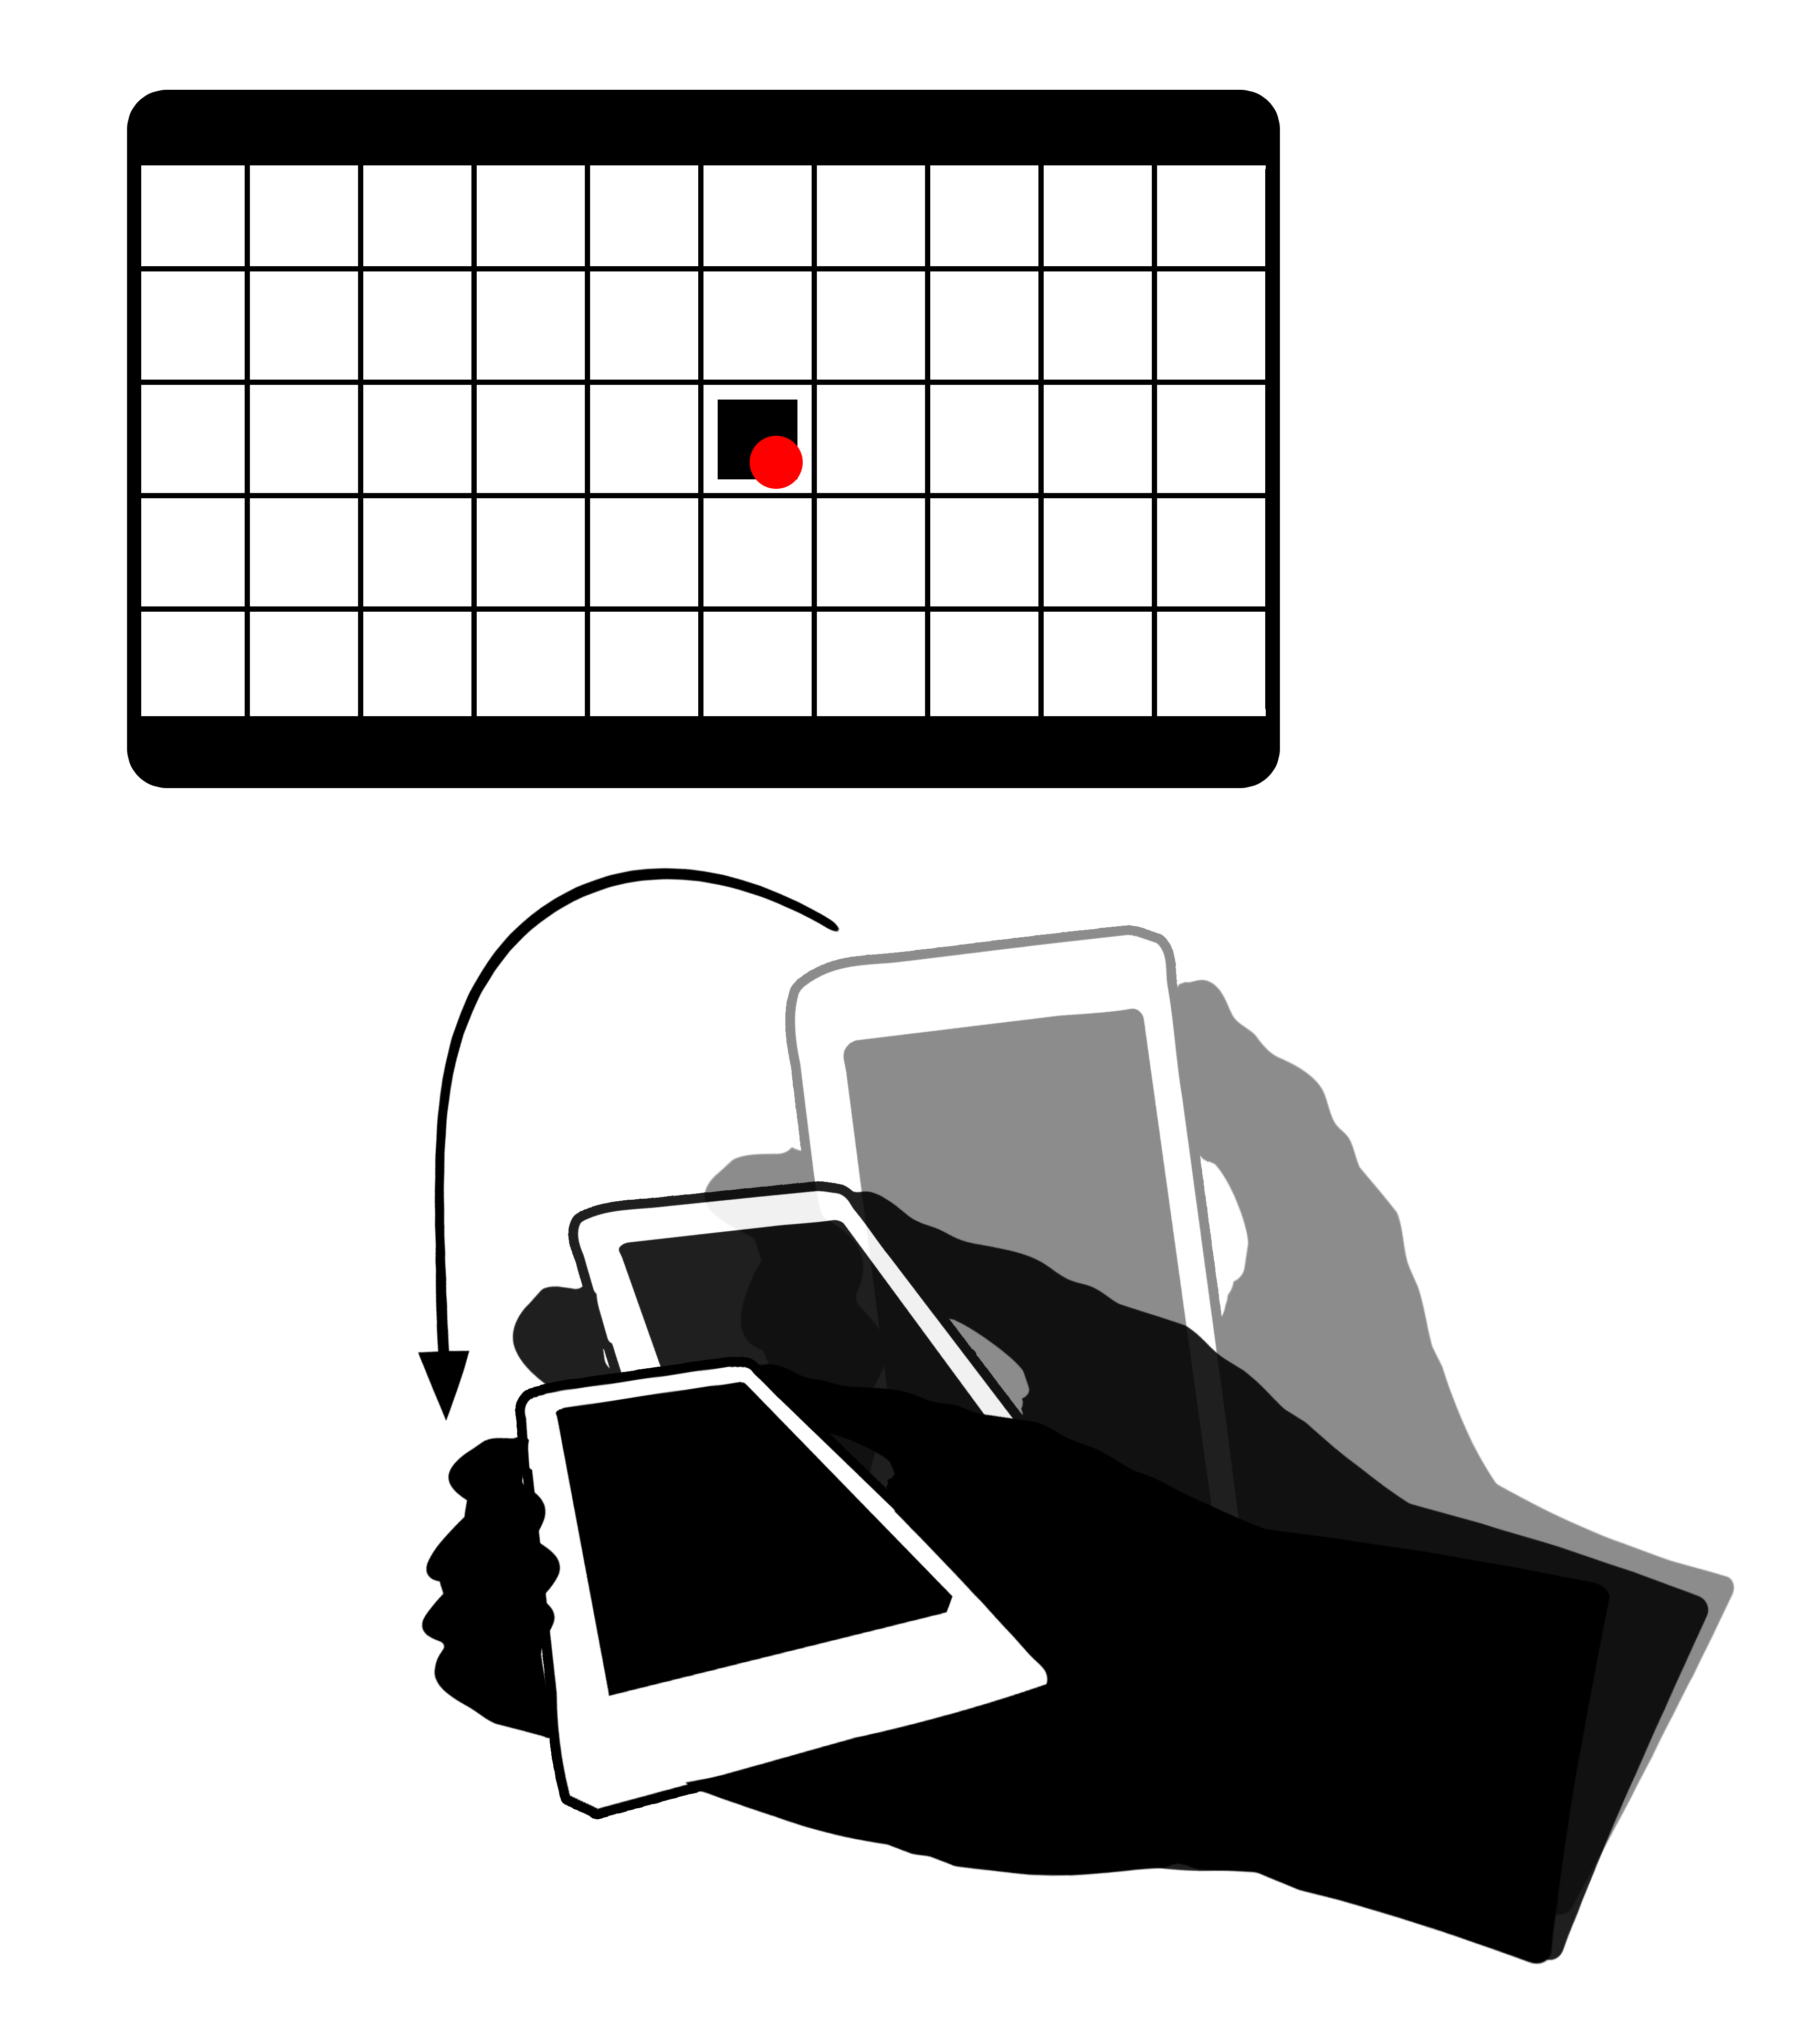
\includegraphics[width = 1\columnwidth]{images/Tilt.jpg}\label{fig:tiltTechnique1}}
\caption{
	\protect\subref{fig:tiltTechnique1} The \tilt technique is performed by doing a forward tilt motion with the phone.
}
\label{fig:tiltTechnique}
\end{figure}

The \throw technique (\Cref{fig:throwTechnique}) is a combination of  
\begin{enumerate*}[label=\itshape\alph*\upshape)]
	\item{a technique for pointing \cite{Scheible:2008} i.e. using a hand as a cursor in mid-air, and}
	\item{a throw technique described by Walter et al. \cite{Walter:2014} and used in a system for sharing information on large public displays.}
\end{enumerate*}
We chose to include this technique based on its natural and playful design.
The technique mimics the real world scenario of throwing something like a ball somewhere or to someone.
\throw is two handed, more complex than aforementioned techniques, and takes a little longer to execute because of the increased number of steps.
The \throw technique is performed by 
\begin{enumerate*}[label=\itshape\roman*\upshape)]
	\item{pointing at a target on the large display with one hand (\cref{fig:throwTechnique})} 
	\item{holding the phone in the other hand, and}
	\item{making a swinging motion towards the large display (\cref{fig:throwTechnique}).}
\end{enumerate*}

\begin{figure}[H]
\subfloat[]{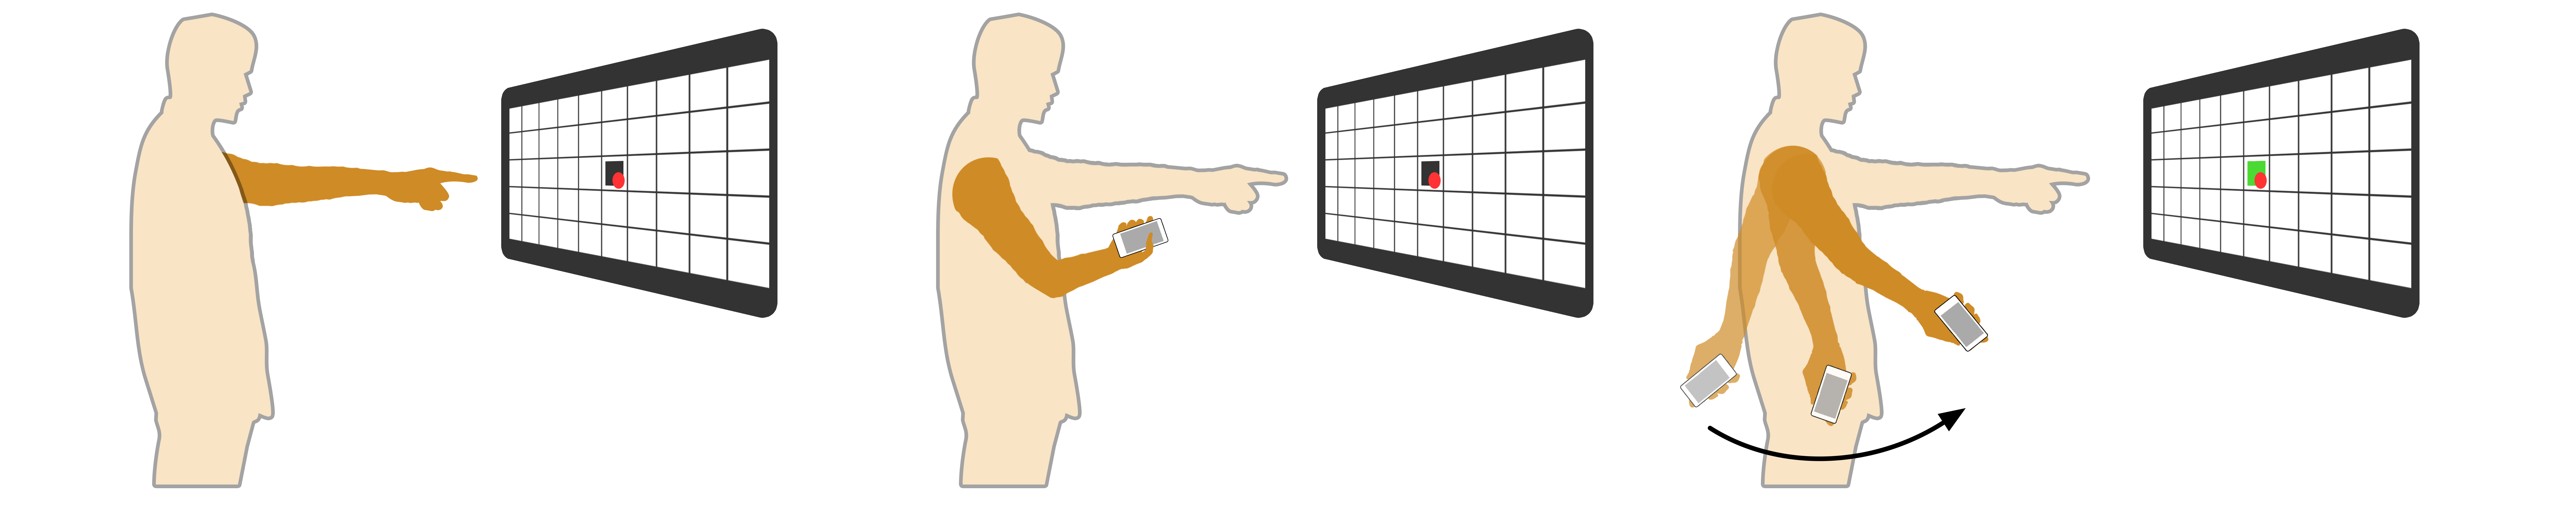
\includegraphics[width = 1\columnwidth]{images/Throw.jpg}\label{fig:throwTechnique1}}
\caption{
	\protect\subref{fig:throwTechnique1} First step of \throw is to point at the screen.
}
\label{fig:throwTechnique}
\end{figure}

The \pinch technique (\Cref{fig:pinchTechnique}) is used in \cite{Ikematsu:2015} by Ikematsu et al., as part of a drag-and-drop method for moving data objects between devices.
Chen et al. uses a pinching gesture in \cite{Chen:2014} for cross-device interaction between a smartphone and a smartwatch to control volume. 
In \cite{Benko:2010}, Benko and Wilson used the \pinch technique for interacting with an omnidirectional dome.
This technique is again a combination of the pointing technique used by Scheible et al. and the aforementioned pinching techniques. 
The reason for including this technique was to imitate the action of picking up a real object e.g. piece of paper, and then moving it to another location.
With \pinch we get a two handed technique which requires the user perform a series of steps and are thus considered more complex and time consuming  than the one handed \swipe and \tilt.
The \pinch technique is performed by 
\begin{enumerate*}[label=\itshape\roman*\upshape)]
	\item{holding the phone in one hand and making a pinch gesture on the phone with the other hand (\Cref{fig:pinchTechnique} 1), subsequently closing the hand}
	\item{pointing at a target on the large display with the closed hand (\cref{fig:pinchTechnique} 2), and}
	\item{opening the hand to complete the technique (\cref{fig:pinchTechnique} 3).}
\end{enumerate*}

\begin{figure}[H]
\subfloat[]{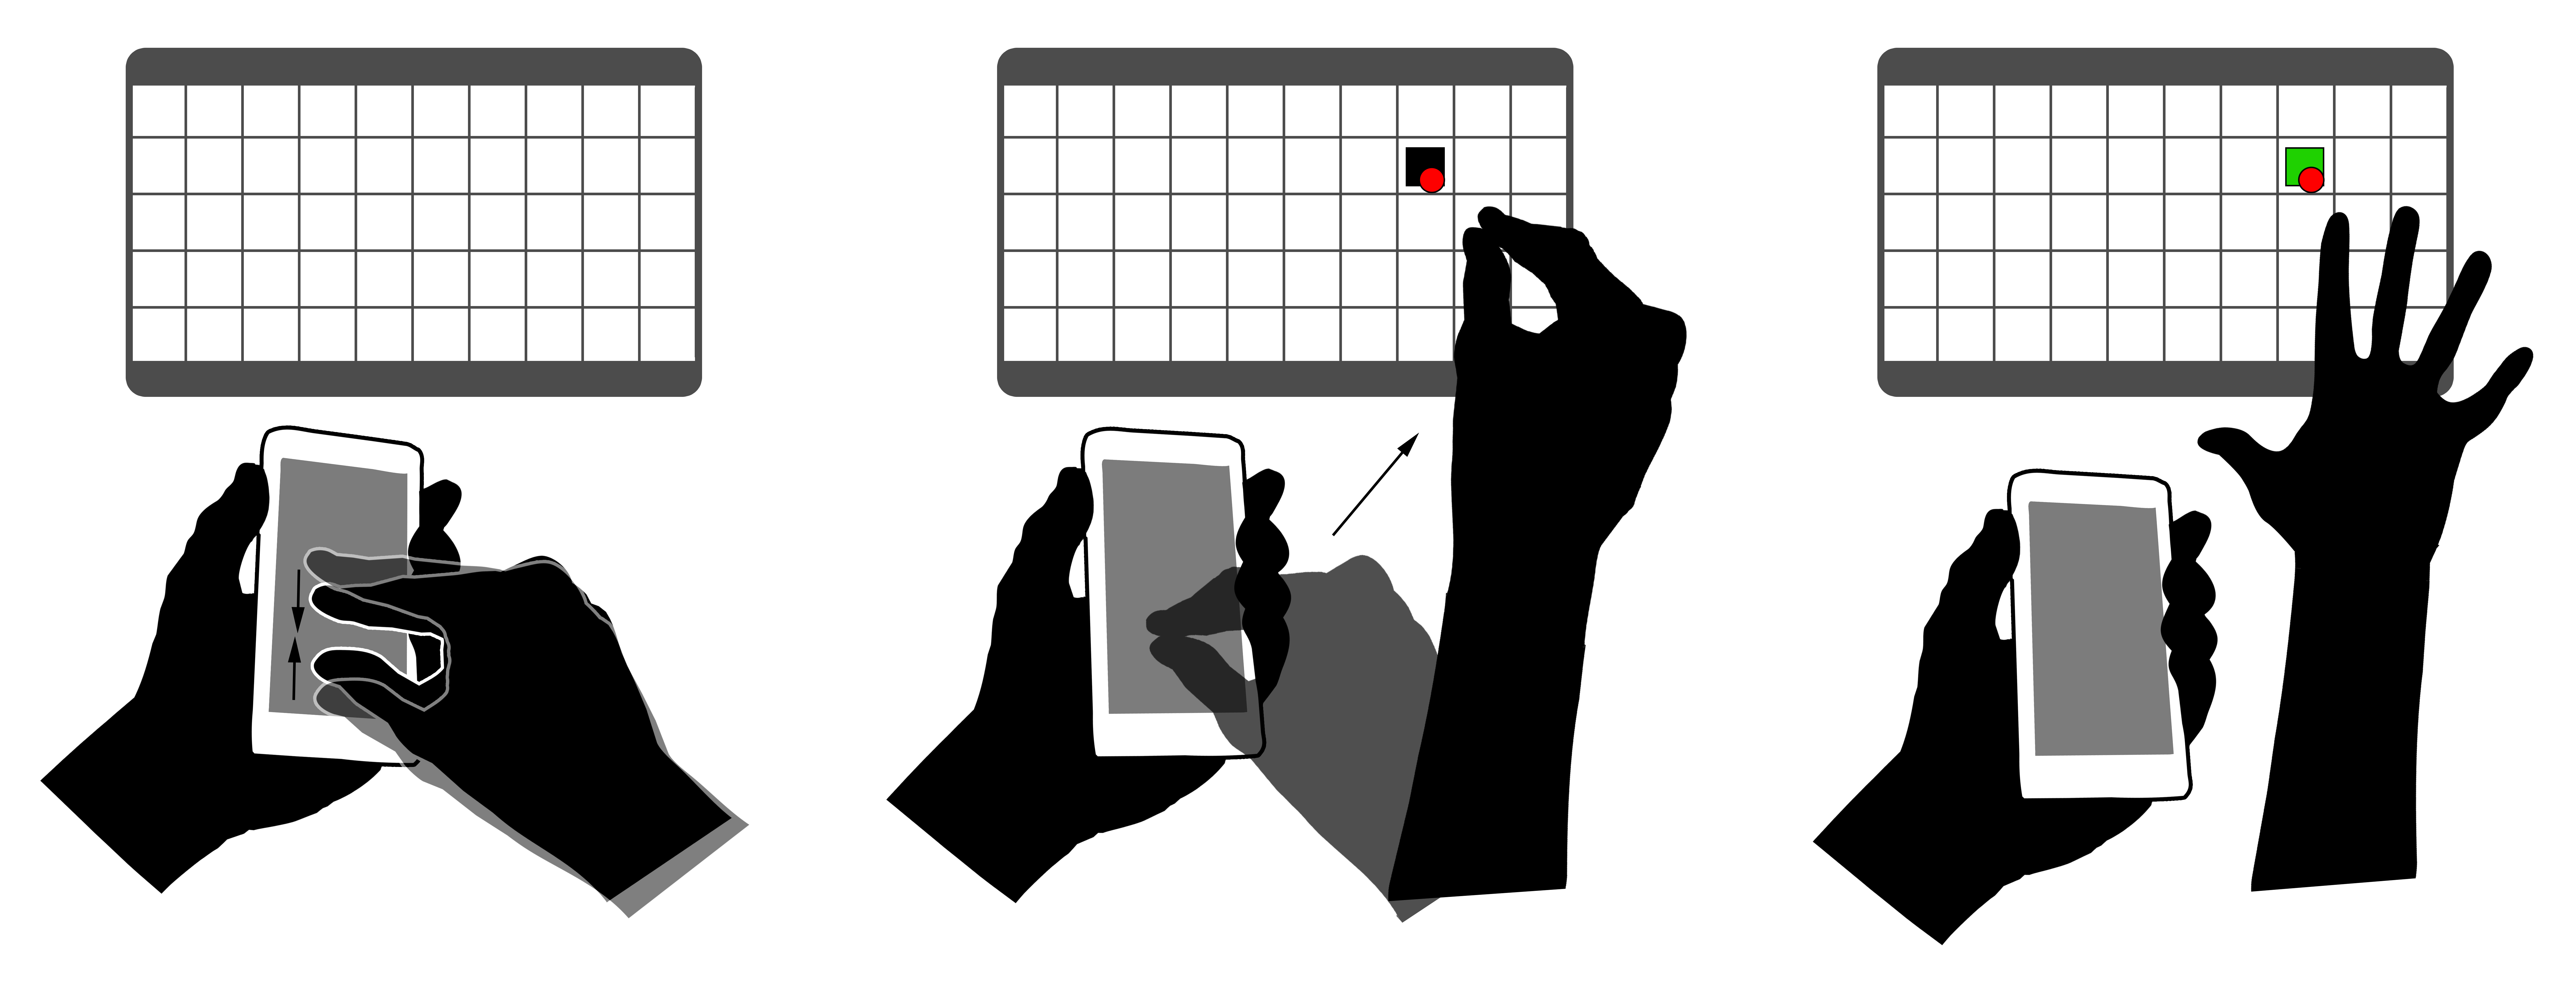
\includegraphics[width = 1\columnwidth]{images/Pinch.jpg}\label{fig:pinchTechnique1}}
\caption{
	\protect\subref{fig:pinchTechnique1} First step of the \pinch technique is to make a pinch gesture on the phone using the index finger and thumb. Second step is to move and use the pinched hand as a pointer.
}
\label{fig:pinchTechnique}
\end{figure}

As mentioned, the techniques have been used in previously published papers where they were part of applications or systems, facilitating interaction between devices such as phone to display interaction and vice versa. 
The described techniques are different in the way they are performed but also the number of hands that are required to make them work.
We chose two techniques that are one-handed (\swipe and \tilt) and two techniques that are two-handed (\throw and \pinch).
Also, to vary the complexity we chose two techniques that require more steps (\throw and \pinch), and two techniques that require less steps for the user to complete the technique (\swipe and \tilt).
% !TEX root = ../paper.tex
\section{Experiment} \label{sec:experiment}
The four cross device interaction techniques mentioned above where implemented and then evaluated in a lab study in order to judge their performance compared to each other.

\subsection{Participants}
In total, 53 people took part in our experiment, which was conducted at Aalborg University's usability lab. The participants where between 20-45 years old (M: 24.4, SD: 4.3) and were between 1.63 and 1.95 meters tall (M: 1.82, SD:7.8). 88.7\% of users were right handed, 90.6\% were male, and 96.2\% of them where smart phone users. Of those who owned smart phones, they had owned one for 2-15 years (M:5, SD:2.1). The participants had several different backgrounds, but a very large part of them were university students. This was not formally recorded. They were recruited through a mixture of our social network, recruitment posters around the campus, and going through group rooms and asking for participants. 

\subsection{Experimental Design}\label{subsec:expdesign}
The experiment was conducted as a withing-subject research, with the four different interaction techniques and two grid sizes as independent variables. For the dependent variables, different measures of completion time and accuracy were used, as well as a small questionnaire in regards to the given interaction technique. Which technique started the test was randomized in order to mitigate the learning effect on the entire set of tests. In the end, the \pinch gesture started 25.4\% of all tests, \swipe started 22.6\% of all tests, \throw started 24.5\% of all tests, and \tilt started 26.4\% of all tests. All of this was automatically logged, and every test session was also video recorded in order to be able to go through them in case we wanted to go into detail in one of the test sessions.

These where the following measures that were logged throughout the experiment: 

\textit{Practice Time:} This was the time each user spent during the practice portion of the experiment for each interaction technique. This was measured as the time from where user started the test for a given interaction technique until the user had hit his 3\ts{rd} target. 

\textit{Total Time:} This was the time each user spent completing the test for a given interaction technique.  This was measured from the time each user had hit his first target after the practice period until he had hit his last target. There were a total of 18 targets, plus the first target. 

\textit{Time per target:} This was the time each user spent hitting each of the target. This was simply measured as the time since each user last hit a target until he hit the current one.

\textit{Accuracy:} Whether or not each user hit the given target. Current pointer and target position (in pixels) were also recorded in order to give a more precise image of accuracy for each test. 

\textit{USE Questionnaire:} Each user was given a questionnaire after having gone through each interaction technique. There were 6 questions, all taken from the USE questionnaire \todo{Create proper reference}. These were asked to get an understanding of how useful and easy to use each technique was. The 6 questions were the following: 

%Arnold M. Lund, Measuring Usability with the USE Questionnaire, STC Usability SIG Newsletter, orginally published in the October 2001 issue (Vol 8, No. 2)
%http://garyperlman.com/quest/quest.cgi?form=USE 

\begin{itemize}
	\item It is easy to use
	\item Using it is effortless
	\item It is easy to learn to use
	\item I can use it successfully every time
	\item I quickly became skillful with it
	\item I learned how to use it quickly
\end{itemize}

User were able to rate their answers to each question on a 7 level Likert scale. We also wrote down any comments we heard during the experiment in order to get a qualitative understanding of each technique.  

\subsection{Implementation}

The 4 implementation techniques mentioned above were implemented in order to push data onto the big display. These four techniques together will be referred to as \textit{push techniques}. They were implemented in a simple and short game, with the combination of a Microsoft Kinect and the accelerometer of the mobile phone used in our experiment. 

Users would control the pointer on the large display with their hands. Which ever hand was closest to the screen would determine the position of the pointer on the large screen. This meant that users could switch hands whenever they pleased at any point during the test. 

The \throw technique was implemented with the help of the Kinect and the accelerometer on the mobile phone. The Kinect would be looking at the user and trying to recognize when a user moved the mobile phone 10 centimeters from behind his midsection to 10 centimeters in front of his midsection, and at the same time detect when a significant change in the accelerometer happened, as to not simply detect a unintentional wave of the arm. It would then use the position of the other hand to see where on the screen the user intended to perform the \throw technique towards. 

The \pinch technique was also implemented with the help of the Kinect and the touch screen on the mobile phone. This technique would start by having the user pinch the shape on the screen of the mobile phone and close his or her hand around it, as if to grab it. The Kinect would then look for a opening of the hand motion, on the pointer hand, and place the given shape at that location. 

The \tilt technique was implemented mostly with the accelerometer of the phone, by listening for a significant change in the x and y axis of the accelerometer, as if tilting the phone forward. The intention here was that the users would point and tilt with the phone, but because of our implementation, it was possible for users to point with one hand and tilt the phone with the other. 

The \swipe technique was implemented with touch screen of the phone. Here, we would detect when a significant swipe would happen on the screen, and then use the pointer location to place the shape that was swiped up onto the screen. Again, because of our implementation, users were capable of pointing with one hand and swiping with the other. 

These four techniques were implemented in a simple target practice game, where the goal was to hit the target with the shown technique and at the same time have selected the correct shape that was displayed on the screen. This was done in order for the user to orient himself with the phone after every technique, and not just simply blindly preform the gesture without paying any attention to the phone at all.  

\subsubsection{The Game}

\todo{Add a picture of the game in progress, with the shapes}

In the game that was created, a grid system is displayed on the large screen, where the each cell of the grid is a square. The grid can take different sizes, having large cells, where the grid is $5 \times 10$ cells, or small cells, where the grid is $10 \times 20$ cells. These will henceforth be referred to as large($5 \times 10$) and small($10 \times 20$) grid.

The game would at random choose one of the four techniques and display a short explanatory film on a screen right beside the main game display. A shape would appear, either a square or a circle, at one of the cells in the grid. This is the target that the participant needs to hit with the given interaction technique. This shape would be chosen at random. 

The user would then have three free tries, in order to get to learn the technique. Only the time that it took the user to come through this practice phase was recorded. The user would have to choose the correct shape on the phone and perform the technique with that shape selected. The shapes on the phone would randomly change positions, so that the user would have to check the phone after every gesture. The grid would also randomly, as far as the user was concerned, change size from large to small or vice-versa. After 19 targets, the test for that specific technique was done, and would then be repeated for the other 3 techniques. 

\subsection{Procedure}

Each test subject was taken into the usability lab and then given a short introduction to what we were doing and why. We would then explain how the system would work and what they had to do. We would hand them a phone, ask them to stand on a marked cross, so that the distance to the screen would always be the same, and start the test.

One of the four techniques would be chosen at random and be presented to the user. A short explanatory movie would be shown on a screen beside the main display showing the user how to perform the technique. The user would then go through the practice period of the test, and then go through the rest of the test, going through a total of 22 targets. The only difference between the two phases was that time was the only measure that was logged during the practice phase of the test. After that, the user would then be asked to fill in a short questionnaire, based on the USE survey, described in the \textbf{Experimental Design} subsection, regarding the technique they just tried. 

This process would be repeated four times in total, one for each technique. After that, we would then ask the test subject to fill in a small demographic survey. We asked them about their age, height, if they were left or right handed, if they had a smart phone, for how long, if they had any experience with a Kinect, Wii, Playstation Move, or any other similar air gesture based technologies, and how often they utilized them. We then thanked them for their time and sent them on their way. The entire test took on average 15 minutes. 
% !TEX root = ../paper.tex
%http://sphweb.bumc.bu.edu/otlt/MPH-Modules/BS/BS704_HypothesisTesting-ANOVA/BS704_HypothesisTesting-Anova_print.html
\section{Results}
We will now present the results that we achieved through out our experiment and also how they were achieved. We will first present our findings in respect to time, then in respect to accuracy. We will then show that there is a significant interaction between our two independent variables, grid size and technique, with regards to success rate. Finally, we will look at the questionnaires and show the significant findings there. We will discuss these results later, in the \nameref{sec:discussion} section.  

\subsection{Target Hit Time}

The four interaction techniques, Pinch, Swipe, Throw and Tilt were completed 18 times per participant. In total, each technique was performed 954 times. \Cref{tab:meanTimesTechnique} shows the mean time per target for each of the techniques as well as their standard deviation. 
\begin{table}[H]
	\centering
	\begin{tabular}{|c|c|c|c|c|}
		\hline
		\rowcolor[HTML]{9B9B9B} 
		 & \textbf{Pinch} & \textbf{Swipe} & \textbf{Throw} & \textbf{Tilt} \\ \hline
		Mean & 8.66  sec         & 5.71 sec          & 7.07 sec          & 6.00 sec         \\ \hline
		Std. Dev. & 6.56 sec & 3.76 sec & 6.08 sec & 3.89 sec \\ \hline
	\end{tabular}
	\caption{Mean time and standard deviation for each technique per target.}
	\label{tab:meanTimesTechnique}
\end{table}

A one way, repeated measure ANOVA revealed, with a Greenhouse-Geisser correction (0.874), that the difference in time per target between the different techniques is in fact a significant($F(2.622, 2498.37)=67.192$, $p<0.001$). A post hoc pair-wise test using a LSD correction revealed that \pinch and \swipe($p<0.001$), \pinch and \tilt ($p<0.001$), \pinch and \throw ($p<0.001$), \swipe and \throw ($p<0.001$), and \throw and \tilt ($p<0.001$) were all significantly different from each other. However, \swipe and \tilt were not ($p=0.092$)

We then examined the effect of grid size on time. Each participant had a equal mixture of small and large grid targets. This means that the four techniques had 9 targets of each size; four large and four small. Every test had 36 targets of each size, totaling 1908 targets of each size, through out all tests. \Cref{tab:meanTimesSize} shows the mean time per target and standard deviation for each grid size. 

\begin{table}[H]
	\centering
	\begin{tabular}{|c|c|c|}
		\hline
		\rowcolor[HTML]{9B9B9B} 
		 & \textbf{Large Grid} & \textbf{Small Grid} \\ \hline
		Mean & 6.21 sec & 7.51 sec \\ \hline
		Std. Dev. & 4.88 sec & 5.71 sec \\ \hline
	\end{tabular}
	\caption{Mean time per target and standard deviation for each grid size per target}
	\label{tab:meanTimesSize}
\end{table}

To determine the effect of grid size on target hit time, we applied another one way, repeated measures ANOVA($F(1,1907) = 77.587$, $p<0.001$). This means that the grid size has a significant effect on time when hitting the target. 

\subsection{Accuracy}

As above, we will perform an analysis on the effect of each technique on accuracy as well as the effect of each grid size. There are the same amount of data points as the above analysis. 

The mean and standard deviation for each technique can be seen in \Cref{tab:meanHitTechnique}. 

\begin{table}[H]
	\centering
	\begin{tabular}{|c|c|c|c|c|}
			\hline
			\rowcolor[HTML]{9B9B9B} 
			& \textbf{Pinch} & \textbf{Swipe} & \textbf{Throw} & \textbf{Tilt} \\ \hline
			Mean & 0.72         & 0.94          & 0.88          & 0.68         \\ \hline
			Std. Dev. & 0.45 & 0.25 & 0.32 & 0.47 \\ \hline
	\end{tabular}
	\caption{Mean hit  and standard deviation for each technique per target.}
	\label{tab:meanHitTechnique}
\end{table}

In order to see the effect of each technique on the hit ratio per target, we performed another one way, repeated measure ANOVA ($F(2.645,2420.246)=105.535$, $p<0.001$), which told us that the different techniques also had a significant effect on the hit ratio. We perform another pair-wise post hoc LSD test to see where the significant differences are. \pinch and \tilt had $p=0.094$, which means that there was no significant difference between these two techniques. All other techniques were significantly different from each other ($p<0.001$). 

We then looked at the grid sizes effect on accuracy. The mean and standard deviation can be seen in \Cref{tab:meanHitSize}. We performed another one-way, repeated measure ANOVA ($F(1,1907)=103.443$, $p<0.001$) to see if the difference between the two grid sizes was significant. The results showed that the two grid sizes had a significant effect on the hit ratio per target. 

\begin{table}[H]
	\centering
	\begin{tabular}{|c|c|c|}
		\hline
		\rowcolor[HTML]{9B9B9B} 
		& \textbf{Large Grid} & \textbf{Small Grid} \\ \hline
		Mean & 0.87 & 0.74 \\ \hline
		Std. Dev. & 0.34 & 0.44 \\ \hline
		\end{tabular}
		\caption{Mean hit and standard deviation for each grid size per target}
		\label{tab:meanHitSize}
\end{table}
% !TEX root = ../paper.tex
\section{Results of Survey}

\begin{figure}[H]
	{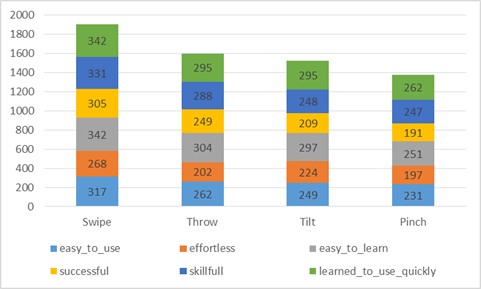
\includegraphics[width = 1\columnwidth , height = 6cm ]{images/survey-data.png}} 
	\caption{
		Cumulative values of survey questions per technique
	}
	\label{fig:allSetup}
\end{figure}
% !TEX root = ../literature.tex
\subsection{Discussion}
%this section needs to be called discussion, and you need to use it to discuss a bit more about the relationships between the different fields, concluding with the idea that some sharing of information across these areas to futher research various aspects would be a good idea. So you are on the right track - but you need to be a bit more detailed in your thinking
This current paper aims to analytically summarize published research within the areas of interaction with large displays, natural user interaction, and cross device interaction.In this section we expand on the relationships between presented different fields, we believe this will further deepen our understanding of them.

%The findings of this work are that gesture recogntion using touchscreens is now a mature enough technology that it is ready for implementation in commerical products. The iPhone has shown that basic gesturing has a place in mobile operating systems and my results show that more complex gestures can be easily recognised and recognised accurately. The problem is context.
By making the objects that surround us change their non-interactive state to a responsive medium, Buxton and Welnner achieved a novelty supporting Weiser's vision of ubiquitous computing. A secondary objective of Weiser was related to the size of the object. An example of this principle can be related to the work of Czerwinski that shows how size can correlate to the performance in a work environment.

A new state is often related to not only a technologically progress but also conceptual ideas. A Technological example would be the development of the Kinect that provide new interaction possibilities\cite{Wilson:2010}, and a conceptual example is to use tangible objects as a medium for interacting with the virtual world\cite{Rekimoto:1997, Keefe:2001}.
This change provides new opportunities and challenges for developing interaction techniques in the interaction space of natural user interaction and cross-device interaction. These two identified areas differ in-between, however they also have common ground, we present this idea in \Cref{fig:litreview}.\\

We reflect upon how the shift from private to public environment correlates with the challenges in natural user interaction and cross-device interaction for interaction techniques.
While there isn't a specific formula covering the creation of an ideal interaction technique, there are some guidances. For example Brignull advices to make the transition between an onlooker to participant less socially awkward. Cheung shows that their are specific barriers for interacting and presents a diagram of each state when said challenges are encountered, he advices that those should be addressed in every case. However we notice that the majority of papers we examined do not explicitly focus on the environment, instead they present unique solutions, without beforehand taking into consideration the settings.
From the research done on public space and public display we are able to identify 3 elements that directly impacts the creation of interaction techniques: \emph{accessibility}, \emph{learn-ability}, and \emph{social acceptance}. To interact with a system it is necessary that the technique can be used without obstacles. For instance a large display can be interacted with by either touch or mid-air gestures, but mid-air gestures risks being interrupted by people who walks between the user and the sensor. It is also important that the user understands how to interact with the system and \emph{``move beyond ephemeral interactions, driven by the playfulness of the interface''}\cite{Jacucci:2010}, especially for a public walk-up-and-use system. However in the end for the user to engage in using the system, the interaction technique must be acceptable in a social circumstances to avoid intimidating or embarrassing the user. 
% The reoccurring challenges for interaction techniques in the public environment are: social acceptability, learning curve, 

With this limitation came different approaches for solving it. 
We identified two different areas which deals with it, we present them in \Cref{fig:litreview}.
\begin{figure}[h!]
\centering
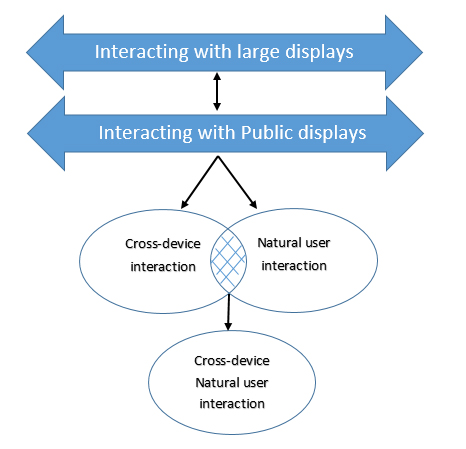
\epsfig{file=images/litreview-fig1.jpg, width=0.5\textwidth}
\caption{Write Caption}
\label{fig:litreview}
\end{figure}
%\todo[inline]{Assuming the numbers are right, then keep this. But for god sake, use cite!}
The fields of natural user interactions and cross-device interactions were examined. 
We were surprised to see that research in combining features from the two areas is slim even though they are complementary to each other. 
There was research that was done [26, 27, 28, 29]. 
Interaction-techniques were evaluated with 3-6 people using qualitative surveys in [27,28,29] and without qualitative surveys in [26].\\

In summary, we can see research opportunities in further exploration of cross-device natural user interactions technique for large displays. We believe the limitations that each of these fields ignore is the interaction space between them. To move beyond this limitation, we believe a unification of these discrete interaction techniques in continuous interaction space and it's further research would be positive and beneficial.
Firstly, as handheld devices become thinner and lighter and spatially-aware technologies, such as Kinect, continue to evolve, this opens a potentially rich space of aforementioned techniques. 
Secondly, we see opportunities in quantitative aspect, for example comparative study of different interaction techniques. 

\section{Conclusion}\label{Sec:Conclusion}
In this paper we presented an overview of HCI research within interacting with large displays. We reviewed 34 papers from the last decade in detail. A picture (\Cref{fig:litreview}) was drawn about the relation of large displays, public displays, cross-device interaction and natural user interaction. Cross device interaction and natural user interaction was found to be a subset of large- and public displays. Based on further examination of these areas in research, we identified cross-device natural user interaction as well as some opportunities and shortcomings that we used to suggest possible future research areas.\\
In the future we would like to see quantitative research within the field of cross-device natural user interaction, as well as use of the produced statistically solid results as a guide for the design of further applications for cross-device interactions and large displays.
% !TEX root = ../paper.tex
\section{Acknowledgments}
\todo[inline]{Acknowledgments here}

%\subsection{References and Citations}
%
%Use a numbered list of references at the end of the article, ordered
%alphabetically by last name of first author, and referenced by numbers
%in
%brackets~\cite{acm_categories,ethics,Klemmer:2002:WSC:503376.503378}.
%Your references should be published materials accessible to the
%public. Internal technical reports may be cited only if they are
%easily accessible (i.e., you provide the address for obtaining the
%report within your citation) and may be obtained by any reader for a
%nominal fee. Proprietary information may not be cited. Private
%communications should be acknowledged in the main text, not referenced
%(e.g., ``[Borriello, personal communication]'').
%
%References should be in ACM citation format:
%\url{http://acm.org/publications/submissions/latex_style}. This
%includes citations to internet
%resources~\cite{acm_categories,cavender:writing,CHINOSAUR:venue,psy:gangnam}
%according to ACM format, although it is often appropriate to include
%URLs directly in the text, as above.


% Use a numbered list of references at the end of the article, ordered
% alphabetically by first author, and referenced by numbers in
% brackets~\cite{ethics, Klemmer:2002:WSC:503376.503378,
%   Mather:2000:MUT, Zellweger:2001:FAO:504216.504224}. For papers from
% conference proceedings, include the title of the paper and an
% abbreviated name of the conference (e.g., for Interact 2003
% proceedings, use \textit{Proc. Interact 2003}). Do not include the
% location of the conference or the exact date; do include the page
% numbers if available. See the examples of citations at the end of this
% document. Within this template file, use the \texttt{References} style
% for the text of your citation.

% Your references should be published materials accessible to the
% public.  Internal technical reports may be cited only if they are
% easily accessible (i.e., you provide the address for obtaining the
% report within your citation) and may be obtained by any reader for a
% nominal fee.  Proprietary information may not be cited. Private
% communications should be acknowledged in the main text, not referenced
% (e.g., ``[Robertson, personal communication]'').

% Balancing columns in a ref list is a bit of a pain because you
% either use a hack like flushend or balance, or manually insert
% a column break.  http://www.tex.ac.uk/cgi-bin/texfaq2html?label=balance
% multicols doesn't work because we're already in two-column mode,
% and flushend isn't awesome, so I choose balance.  See this
% for more info: http://cs.brown.edu/system/software/latex/doc/balance.pdf
%
% Note that in a perfect world balance wants to be in the first
% column of the last page.
%
% If balance doesn't work for you, you can remove that and
% hard-code a column break into the bbl file right before you
% submit:
%
% http://stackoverflow.com/questions/2149854/how-to-manually-equalize-columns-
% in-an-ieee-paper-if-using-bibtex
%
% Or, just remove \balance and give up on balancing the last page.
%
\balance{}

% REFERENCES FORMAT
% References must be the same font size as other body text.
\bibliographystyle{SIGCHI-Reference-Format}
\bibliography{paper}

\end{document}

%%% Local Variables:
%%% mode: latex
%%% TeX-master: t
%%% End:
